
\section{Tag-based Genetic Regulation}
\label{chapter:tag-based-regulation:sec:tag-based-genetic-regulation}

Here, we allow programs to use tag-based referencing to dynamically regulate module execution.
To achieve this, we draw inspiration from both natural and artificial gene regulatory networks. 
We demonstrate that this approach promotes more effective solutions for context-dependent problems.

% - gene regulation background, briefly -
Gene regulatory networks represent the complex interactions among genes, transcription factors, and signals from the environment that, together, control gene expression \citep{banzhaf_artificial_2015}.
Gene regulation allows for feedback loops so that prior events can continue to influence future expression in flexible and nuanced ways. 
Gene regulation underlies most important biological processes, including cell differentiation, metabolism, the cell cycle, and signal transduction \citep{karlebach_modelling_2008}.
The role of gene regulatory networks in sustaining complex life has inspired varied and abundant computational models of these networks \citep{karlebach_modelling_2008,cussat-blanc_artificial_2019}.

% ---- BEGIN REVISION ----
Artificial gene regulatory networks have been used to study how natural gene regulation evolves \citep{aldana_robustness_2007,crombach_evolution_2008,draghi_evolutionary_2009} and as a tool in evolutionary computation to solve challenging control problems (as reviewed by \citep{cussat-blanc_artificial_2019}).
Evolved artificial gene regulatory networks have even been used as indirect encoders, providing a developmental phase to translate genomes into programs \citep{banzhaf_artificial_2003,lopes_regulatory_2012} or neural networks \citep{kowaliw_using_2014}.
La Cava \textit{et al.} demonstrated a form of \textit{epigenetic} regulation for genetic programming where ``gene'' activation and silencing is learned each generation \citep{la_cava_genetic_2015,la_cava_inheritable_2015}; however, the programs themselves did not have direct control over these regulatory elements.
% @AML: new sentence below
Inspired by chromatin remodeling in biological cells, Turner \textit{et al.} introduced artificial epigenetic networks that allow for the regulation (\textit{i.e.}, the addition or removal) of internal network components  \citep{turner_artificial_2017}; such topological self-modification improved problem-solving success for dynamical control problems.
% ---- END REVISION ----

% ----- REVISIONS BEGIN -----
We aim to incorporate gene regulatory network-inspired methodology to allow programs to dynamically adjust which module is triggered by a particular call based on not just current inputs, but also prior inputs.
We achieved this goal by instantiating gene regulatory networks using tag-based referencing.
Specifically, we implemented tag-based genetic regulation in the context of the linear GP system SignalGP \citep{lalejini_evolving_2018}, which is described in further detail in Section \ref{chapter:tag-based-regulation:sec:methods:signalgp}.
Here, we describe tag-based genetic regulation in terms of our SignalGP-based implementation; however, our overall approach is immediately applicable to each of the tag-enabled systems described in Section \ref{chapter:tag-based-regulation:sec:tag-based-referencing} and can be easily incorporated into any genetic programming representation.

Briefly, programs in SignalGP are composed of tag-addressed modules (\textit{i.e.}, functions), each of which contain a linear sequence of instructions. 
Each instruction has arguments, including an evolvable tag that can be used to identify and call a tag-addressed module.
When a referring tag (\textit{e.g.}, from an instruction) is used to look up a tag-addressed module, all modules in that program are ranked according to a tag-matching score. 
A tag-matching score quantifies the quality of the reference between a referring tag and a module's tag; we always select the module with best reference quality (\textit{i.e.}, the highest tag-match score with the referring tag).
When a module is called, it is executed procedurally, instruction-by-instruction, in the same way as in a conventional linear GP system. 

\begin{figure}[ht!]
    \centering
    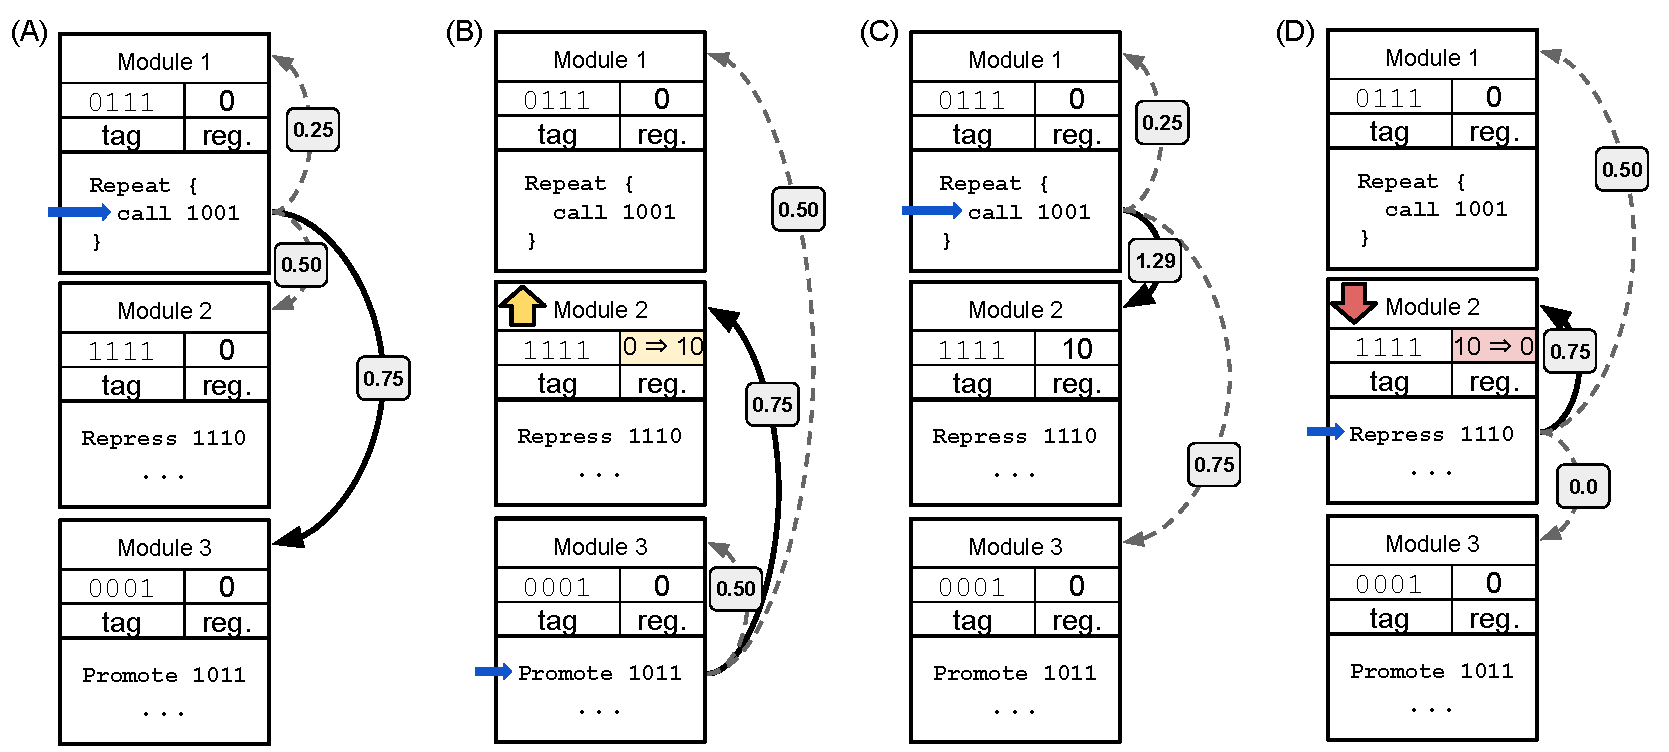
\includegraphics[width=\textwidth]{chapters/05-tag-based-genetic-regulation/media/regulation-example.pdf}
    \caption{\small
    \textbf{Tag-based genetic regulation example.}
    This example depicts a simple oscillating regulatory network instantiated using tag-based regulation.
    In this example, tags are length-4 bit strings. 
    The ``raw'' match score between two tags equals the number of matching bits between them.
    Regulation (reg.) modifies match scores for ``\code{call}'' instructions according to Equation \ref{chapter:tag-based-regulation:equ:reg-transform}.
    First (A), the \code{call 1001} in Module 1 executes, triggering Module 3. 
    Next (B), Module 3 is executed, promoting Module 2. 
    After Module 3 returns, the \code{call 1001} in Module 1 executes again (C); however, Module 2's promotion causes it to be triggered instead of Module 3. 
    Finally (D), Module 2 executes and represses itself, resetting its regulatory modifier to 0. 
    }
    \label{chapter:tag-based-regulation:fig:regulation-example}
\end{figure}


% Revision
We modified SignalGP in two ways to implement tag-based genetic regulation: 

\begin{enumerate}
    \item We added a ``regulatory modifier'' value (represented as a floating point value) to all tag-addressed modules. A module's regulatory modifier adjusts how well that module will match to referring tags, and thus, the likelihood it will be referenced.
    \item We supplemented the instruction set with promoter and repressor instructions that, when executed, adjust a target module's regulatory modifier. 
\end{enumerate} 

When a program begins execution, each internal module initially has no regulatory modification\footnote{
    Alternatively, allowing programs to inherit their parent's regulatory modifiers can provide a simple model of epigenetics.
}.
When a promoter or repressor instruction is executed, its associated tag identifies which module should be regulated using tag-based referencing.
Promoter instructions increase a target module's regulatory modifier, which increases the module's tag-match score with subsequent references (according to equation \ref{chapter:tag-based-regulation:equ:reg-transform} below) and thus increases the module's chances of being referenced.
Repressor instructions have the opposite effect.
Regulatory modifiers can be configured to persist over a program's entire execution or passively decay over time.
% passively decay over time or persist over a program's entire execution.

When determining which module to call at runtime, each module's tag-match score is a function of how well the module's tag matches the call instruction's tag as modified by the module's regulatory value.
% @AML: This next sentence (or two) is in rough shape, need streamlining.
If a module's regulatory modifier has been sufficiently decreased by repressor instructions, it is possible that the module will no longer be able to be referenced, as its regulated tag-match score will always be lower than that of all other program modules. 
To avoid such an unrecoverable regulatory state, promoter and repressor instructions use \textit{unregulated} tag-based referencing to identify which modules they regulate; that is, we do not apply regulatory modifiers to tag-based references made by promoter and repressor instructions. 
This ensures that no matter how much a particular module has been repressed, subsequent promoter instructions can increase its regulatory modifier.
Figure \ref{chapter:tag-based-regulation:fig:regulation-example} gives a simplified example of how promoter and repressor instructions can dynamically adjust module execution over time.

We have implemented a toolbox of interchangeable methods for applying regulation to tag-matching scores in the Empirical library \citep{charles_ofria_2020_empirical}. 
Here, we use a simple exponential function to apply a module's regulation modifier to its tag-match score calculations: 

\begin{equation}
M_{r}(t_q, t_m, R_m) = M(t_q, t_m) \times b^{R_m}
\label{chapter:tag-based-regulation:equ:reg-transform}
\end{equation}

\noindent
$R_m$ specifies the module's regulation modifier, which is under the direct control of the evolving programs.
$M_r$ is the regulation-adjusted match score between a querying tag ($t_q$) and the module's tag ($t_m$).
$M$ is a function that gives the baseline, unadjusted match score between the querying tag and module tag.
If tags are represented as floating point values, $M$ can be as simple as the absolute difference between the two tags.
%; in this work, tags are represented as bit strings, and $M$ is computed using the Streak metric \citep{downing_intelligence_2015}.
The strength of regulation is determined by the constant, $b$ (set to $1.1$ in this work). 

\begin{figure}[htbp]
    \centering
    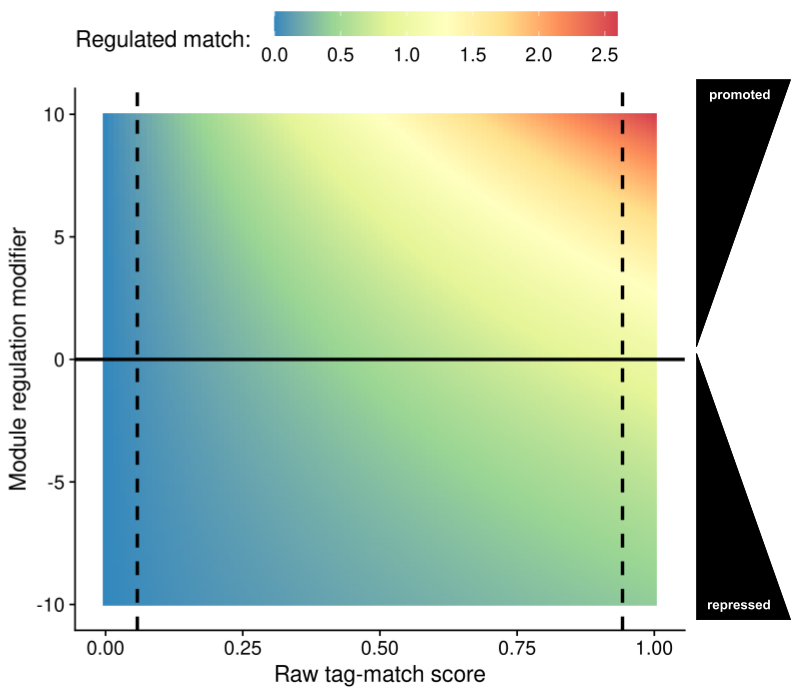
\includegraphics[width=0.6\columnwidth]{chapters/05-tag-based-genetic-regulation/media/expontential-regulation.png}
    \caption{\small
    \textbf{Regulated tag-match score as a function of raw tag-match score and regulatory modifier values according to Equation \ref{chapter:tag-based-regulation:equ:reg-transform}.}
    The horizontal black line indicates a neutral regulatory state; 
    repressed states are below the line, and promoted states are above the line.
    We expect the raw tag-match score (calculated using the Streak similarity metric, which is described later in Section \ref{chapter:tag-based-regulation:sec:methods:signalgp}) of 90\% of random pairs of tags to fall between the two dashed vertical lines; to compute the location of these lines, we generated $10^{5}$ pairs of random tags and found the region that contained the middle 90\% of raw tag-matching scores.
    }
    \label{chapter:tag-based-regulation:fig:exponential-regulation-function}
\end{figure}

When determining which module to reference, each candidate module's $M_r$ is computed, and the module with the highest $M_r$ value is chosen. 
Intuitively, modules with $R_m < 0$ are down-regulated (\textit{i.e.}, in a repressed state), modules with $R_m > 0$ are up-regulated (\textit{i.e.}, in a promoted state), and modules with $R_m = 0$ are unmodified by regulation. 
That is, down-regulated modules have lower tag-match scores than they otherwise would without regulation, and up-regulated modules have higher tag-match scores than they otherwise would without regulation.
Figure \ref{chapter:tag-based-regulation:fig:exponential-regulation-function} gives a visual representation of Equation \ref{chapter:tag-based-regulation:equ:reg-transform}.

In preliminary experiments, we tested several different methods of implementing regulation (including additive, multiplicative, and the current exponential techniques).
We found no evidence for any one method performing substantially better than the others.
Future work will more thoroughly explore the potential effects of different regulation mechanisms. 

% ----- REVISIONS END -----






